Nesta Seção são apresentados experimentos repetidos a exaustão para avaliar o desempenho médio esperado do sistema. E também outros experimentos preliminares.

\section{Comparação SEIF vs Odometria}
\label{sec:exp-estimate-comparison}
Este primeiro experimento visa medir a capacidade do SEIF para estimar a 
pose do robô enquanto ele explora o ambiente de maneira autônoma, 
mediante comparação da estimativa 
com a odometria das rodas. Além disso, compara-se a estimativa do SEIF 
variando a cardinalidade do conjunto de \textit{landmarks} 
ativas $\{\bupvec{m}{+}\}$. O critério de comparação utilizado foi o 
Integral do Erro Absoluto (IAE) (Equação \ref{eq:iae-error}) da posição estimada $\bvec{\hat{x}}$, em 
relação à pose real $\bvec{x}$ colhida do simulador. Para repetir o experimento com outro tamanho de $\{\bupvec{m}{+}\}$ foram gravadas a sequência de entradas $\bsubvec{u}{1:t}$ 
(posição angular das rodas) e a sequência de leituras $\bsubvec{y}{1:t}$ 
do sensor LiDAR.
\begin{equation}
  \IAE(\bvec{\hat{x}}, \bvec{x}) = \int{
    \sqrt{(\hat{x} - x)^2 + (\hat{y} - y)^2} \, \partial t
  }
  \label{eq:iae-error}
\end{equation}
em que: \begin{itemize}
  \item $(x, y)$ são as componentes de posição do estado real $\bvec{x}$ do agente
  \item $(\hat{x}, \hat{y})$ são as componentes de posição do estado estimado $\bvec{\hat{x}}$
\end{itemize}

A Tabela \ref{table:iae} lista os valores obtidos para o IAE e a Figura \ref{fig:iae} ilustra a evolução 
temporal do erro da estimativa de posição do robô. Além 
da posição, também foi avaliada a evolução do erro na estimação da 
orientação, ilustrado na Figura \ref{fig:theta-error}. Em ambas as 
Figuras, os valores obtidos pelo SEIF são mostrados separadamente, pois aparecem sobrepostos na escala do erro da odometria.

\begin{table}[]
\caption{Integral do Erro Absoluto da trajetória do robô para diferentes estimadores}
\label{table:iae}
\center
\begin{tabular}{cc}
\hline
Fonte da estimativa & $\IAE$ (m) \\ \hline
Odometria & 846.01 \\
SEIF $\bupvec{m}{+} = 4$ & \textbf{7.01 }\\
SEIF $\bupvec{m}{+} = 8$ & 8.04 \\ \hline
\end{tabular}
\end{table}

\begin{figure}
  \centering
  \begin{subfigure}{.75\textwidth}
    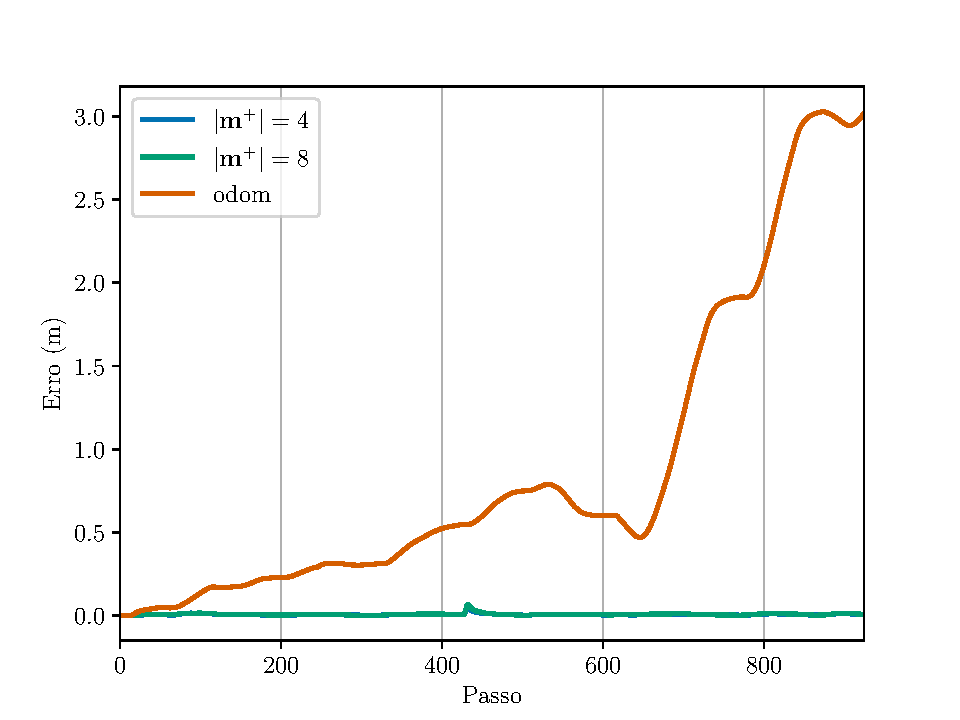
\includegraphics[width=\textwidth]{figs/iae-odom-seif.pdf} 
    \caption{Evolução temporal do erro da estimativa de posição pela odometria e duas configurações do SEIF com $\lvert \bupvec{m}{+}\rvert = 4 $ e $\lvert \bupvec{m}{+}\rvert = 8 $.}
    \label{fig:iae-odom-and-seifs}
  \end{subfigure}
  \begin{subfigure}{.75\textwidth}
    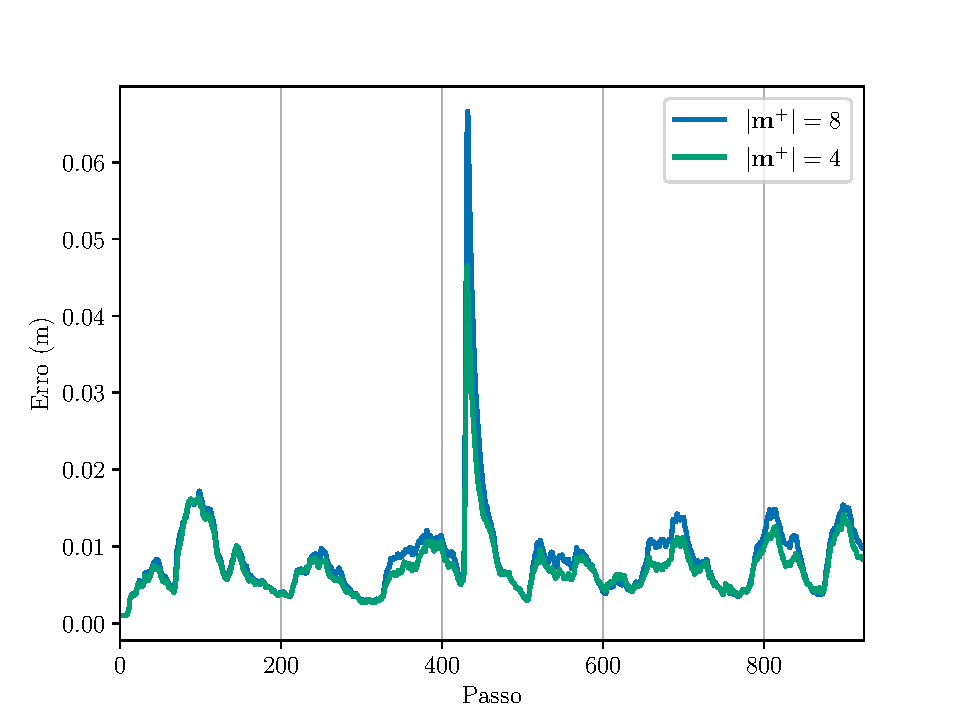
\includegraphics[width=\textwidth]{figs/iae-seifs.pdf} 
    \caption{Evolução temporal do erro da estimativa de posição pelas duas configurações do SEIF com $\lvert \bupvec{m}{+}\rvert = 4 $ e $\lvert \bupvec{m}{+}\rvert = 8 $.}
    \label{fig:iae-seifs}
  \end{subfigure}
  \caption[Erros de estimação da posição do robô no experimento SEIF vs Odometria]{Erros de estimação da posição do robô durante exploração parcial do ambiente da Figura \ref{fig:environment}}
  \label{fig:iae}
\end{figure}

\begin{figure}
  \centering
  \begin{subfigure}{.75\textwidth}
    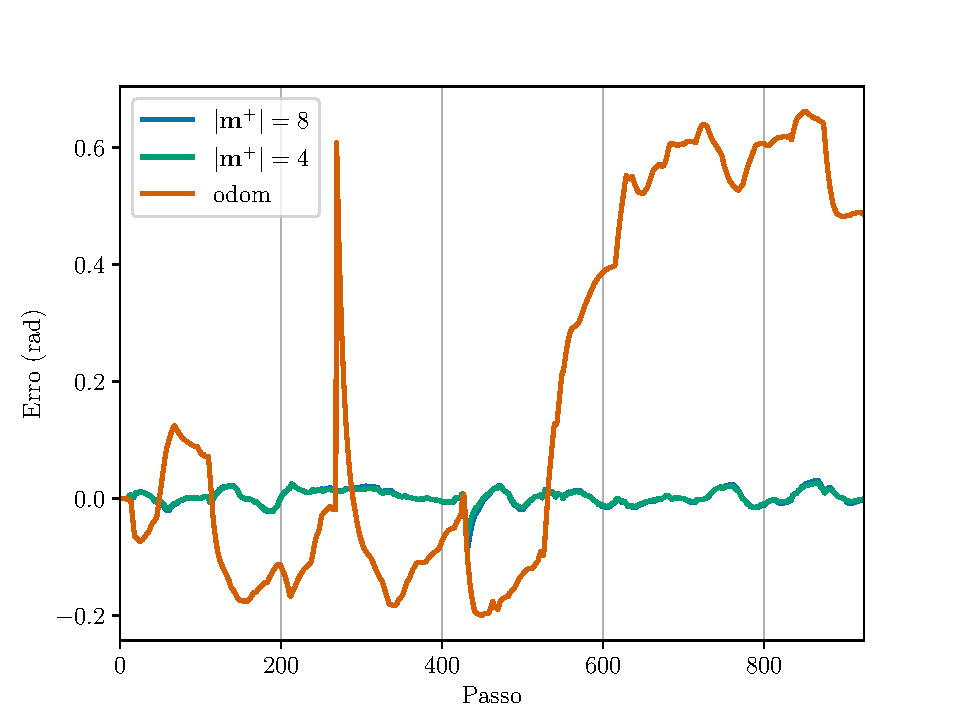
\includegraphics[width=\textwidth]{figs/theta-error-odom-seif.pdf} 
    \caption{Evolução temporal do erro da estimativa de orientação do robô pela odometria e pelas duas configurações do SEIF com $\lvert \bupvec{m}{+}\rvert = 4 $ e $\lvert \bupvec{m}{+}\rvert = 8 $.}
    \label{fig:theta-error-odom-and-seifs}
  \end{subfigure}
  \begin{subfigure}{.75\textwidth}
    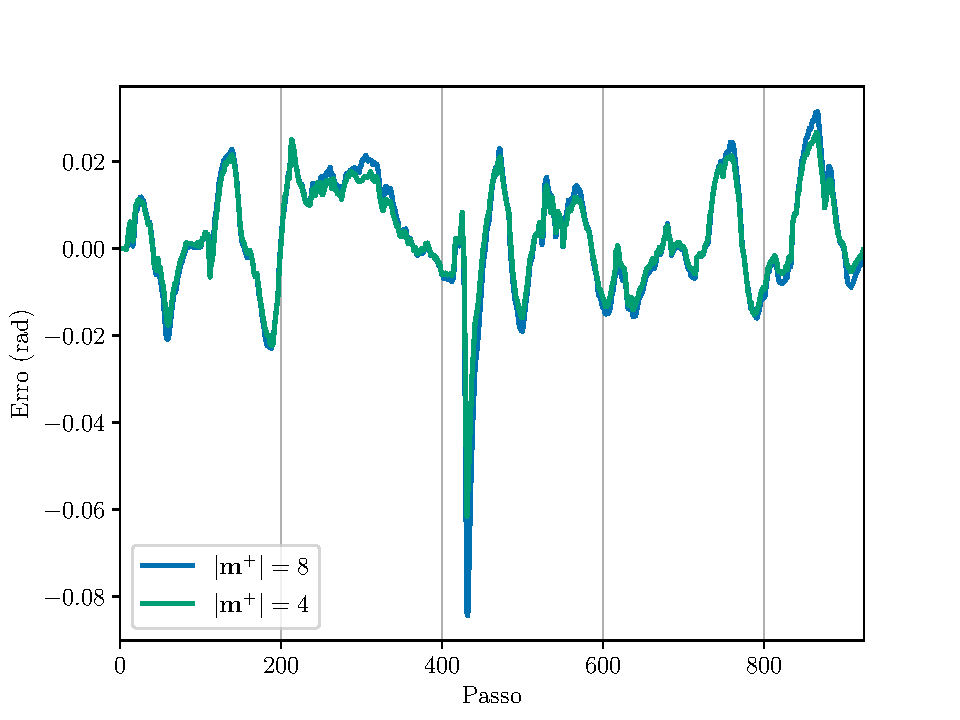
\includegraphics[width=\textwidth]{figs/theta-error-seifs.pdf} 
    \caption{Evolução temporal do erro da estimativa da orientação do robô pelas duas configurações do SEIF com $\lvert \bupvec{m}{+}\rvert = 4 $ e $\lvert \bupvec{m}{+}\rvert = 8 $.}
    \label{fig:theta-error-seifs}
  \end{subfigure}
  \caption[Erros de estimação de orientação no experimento SEIF vs Odometria]{Erros de estimação da orientação do robô durante exploração parcial do ambiente da Figura \ref{fig:environment}}
  \label{fig:theta-error}
\end{figure}

Como esperado, ambas as configurações do SEIF estimaram 
de maneira satisfatória tanto a posição quanto a 
orientação do robô quando comparadas com a estimação da 
odometria. Porém, nota-se que a configuração com 
a cardinalidade do conjunto $\{\bupvec{m}{+}\}$ menor estimou 
melhor tanto a posição quanto a orientação, o que vai 
contra o consenso geral e a observação de \citeonline[p.~408]{thrun2005probabilistic} de que quanto maior o conjunto 
$\bupvec{m}{+}$ melhor é a estimativa. A causa dessa divergência não foi 
entendida até o momento da escrita deste texto; além disso, precisa ser 
verificada de maneira sistemática através de repetidas simulações.

\section{Comparações sobre uso de memória}
Neste experimento foram comparados o uso de memória de diferentes 
configurações do SEIF num mapa com 36 \textit{landmarks} com 
o uso que a abordagem mais clássica EKF-SLAM utilizaria. Nesse ensaio o 
robô foi teleoperado, e para garantir a reprodução exata do mesmo cenário 
as entradas e leituras foram novamente gravadas para alimentar as 
diferentes configurações do SEIF.

As quantidades de elementos não nulos da matriz de informação de cada 
parametrização estão compiladas na Tabela \ref{table:memory-usage} e um 
comparativo com a quantidade de memória que seria utilizado pelo EKF-SLAM, 
com a mesma quantidade de \textit{landmarks}, é ilustrado na Figura \ref{fig:seif-memory-usage}. Por fim, as matrizes de informação são mostradas na 
Figura \ref{fig:seif-info-matrix-memory} para ilustrar 
sua estrutura e quantidade de elementos nulos, que não ocupam 
memória quando utilizada uma estrutura de dados adequada para a representação 
de matrizes esparsas.

O perfil de uso de memória observado mostrou-se como esperado; quanto maior 
a cardinalidade do conjunto de \textit{landmarks} ativas $\bupvec{m}{+}$, maior o 
consumo de memória pelo SEIF-SLAM. Além disso, todas as parametrizações 
usam muito menos memória quando comparados com o EKF-SLAM.

\newcolumntype{Y}{>{\centering\arraybackslash}X}
\begin{table}[]
\centering
\caption{Quantidade de elementos não nulos da matriz de informação esparsa para diferentes configurações do SEIF-SLAM}
\label{table:memory-usage}
\begin{tabularx}{\textwidth}{@{}YYY@{}}
\hline
Cardinalidade do conjunto $\{\bupvec{m}{+}\}$ & Elementos não nulos da matriz de informação & 
Economia em relação ao EKF-SLAM\footnotemark{} \\ 
\hline
2 & 1721 & 69.40\% \\
4 & 1879 & 66.60\% \\
8 & 2021 & 64.07\% \\
\hline
\end{tabularx}
\end{table}

\footnotetext{Embora esses valores correspondam ao número de elementos nulos em relação ao tamanho total da matriz de informação, eles não representam necessariamente economia de memória. Para que a matriz esparsa seja representada é necessário utilizar memória extra para organizar o espaço de armazenamento dos elementos. Porém, essa quantidade tende a ser irrisória quando comparada com a quantidade total de elementos de uma matriz densa. Na estrutura de dados utilizada nesse trabalho, a quantidade de memória utilizada para armazenar a matriz esparsa é da ordem de $\bigO{2n + N}$, onde $n$ é a quantidade de elementos não nulos e $N$ é a dimensão da matriz. Porém, esses valores podem variar dependendo da técnica utilizada para armazenar a matriz.}

\begin{figure}
  \centering
  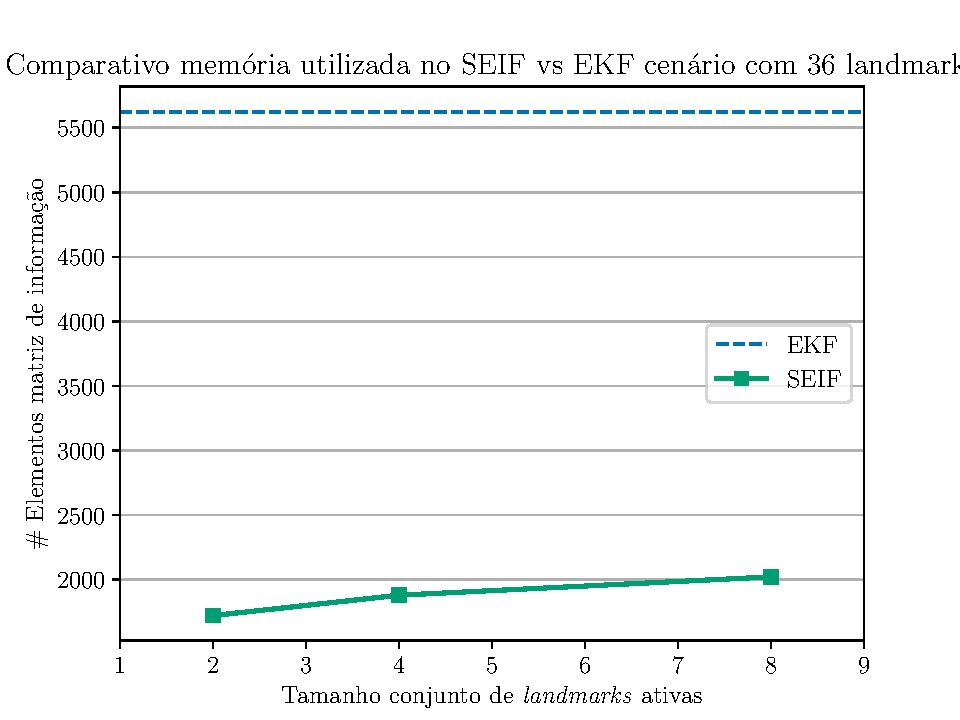
\includegraphics[width=0.7\textwidth]{figs/seif-memory-usage.pdf}
  \caption[Comparação do uso de memória pelo Filtro de Informação Estendido Esparso em relação ao Filtro de Kalman Estendido]{Uso de memória para diferentes parametrizações do SEIF-SLAM com diferentes tamanhos (2, 4, 8) do conjunto de \textit{landmarks} ativas. A linha tracejada representa a quantidade de elementos que a matriz do EKF-SLAM teria para o mesmo cenário.}
  \label{fig:seif-memory-usage}
\end{figure}

\begin{figure}
  \centering
  \begin{subfigure}{0.49\textwidth}
    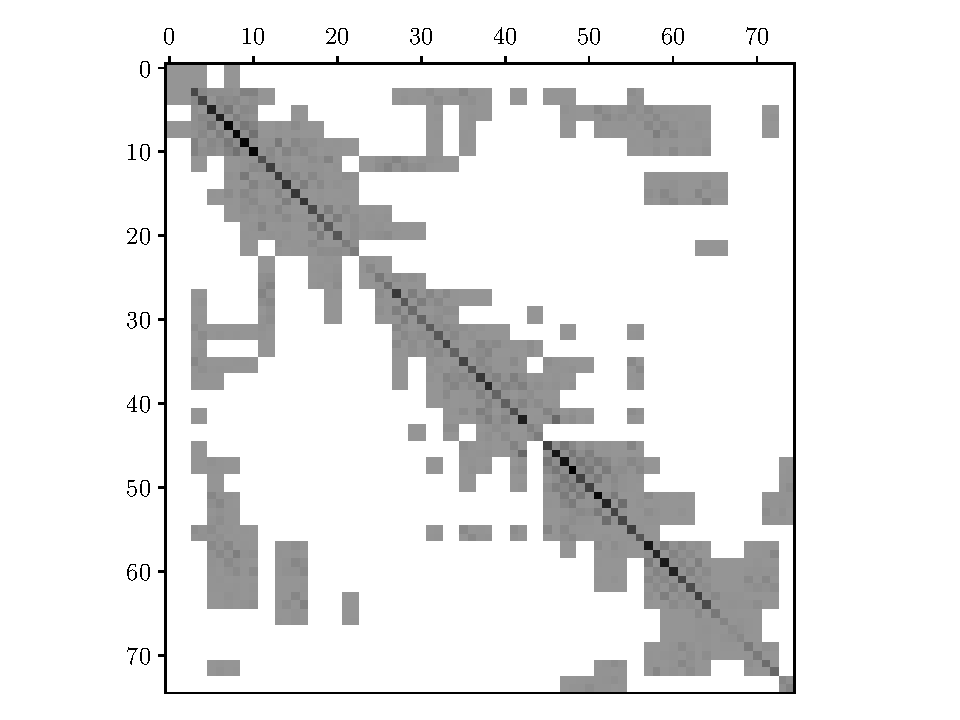
\includegraphics[width=\textwidth]{figs/seif-2-info-matrix.pdf} 
    \caption{$\lvert\{ \bupvec{m}{+} \}\rvert = 2$}
    \label{fig:seif-info-matrix-02}
  \end{subfigure}
  \hfill
  \begin{subfigure}{0.49\textwidth}
    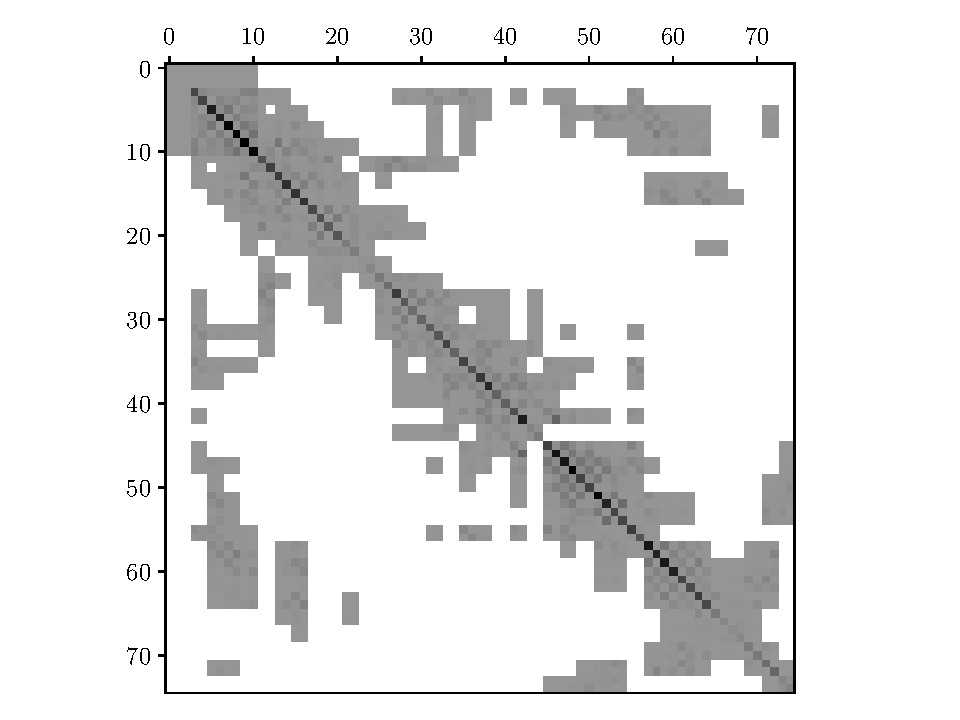
\includegraphics[width=\textwidth]{figs/seif-4-info-matrix.pdf} 
    \caption{$\lvert\{ \bupvec{m}{+} \}\rvert = 4$}
    \label{fig:seif-info-matrix-04}
  \end{subfigure}
  \begin{subfigure}{0.49\textwidth}
    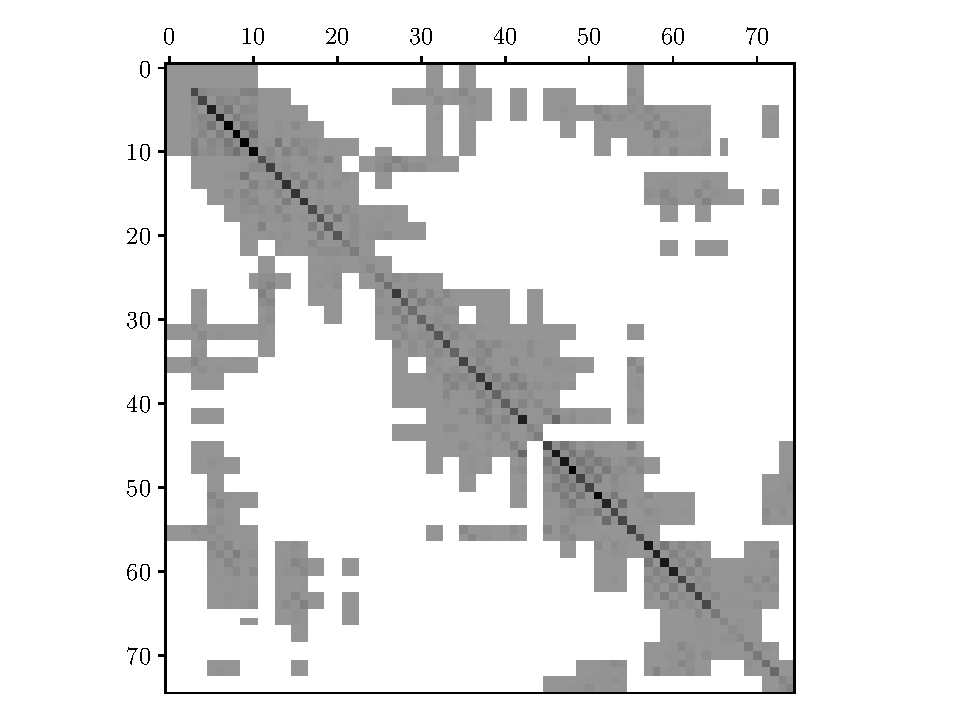
\includegraphics[width=\textwidth]{figs/seif-8-info-matrix.pdf} 
    \caption{$\lvert\{ \bupvec{m}{+} \}\rvert = 8$}
    \label{fig:seif-info-matrix-08}
  \end{subfigure}
  \caption[Matrizes de informação resultantes de diferentes valores de cardinalidade do conjunto de \textit{landmarks} ativas]{Representação das matrizes de informação correspondentes aos experimentos da Tabela \ref{table:memory-usage}. Os elementos nulos são representados pela cor branca, e os não nulos em escala de cinza. Quanto mais escuro o tom de cinza, maior a magnitude do valor representado.}
  \label{fig:seif-info-matrix-memory}
\end{figure}


\section{Desempenho de mapeamento de um único agente}
\label{sec:exp-single-robot}
Para avaliar o desempenho de mapeamento de dois ou mais agentes 
resolvendo o problema SLAM de maneira distribuída e descentralizada, 
primeiro é necessário entender o desempenho de um único agente 
resolvendo a mesma tarefa para assim possuirmos uma base de comparação.

Para isso um único agente foi submetido, repetidamente, à tarefa de mapeamento do ambiente apresentado na Figura \ref{fig:environment}. 
Cada uma dessas simulações poderia assumir um dos seguintes resultados:
\begin{enumerate}
  \item \textbf{Sucesso}: o robô conseguiu mapear 90\% ou mais da área sem 
  divergência na estimação de sua posição dentro de um tempo limite estipulado.
  \item \textbf{Falha por tempo limite excedido}: O robô não conseguiu mapear ao 
  menos 90\% da área antes do limite de tempo (foram dados 17 
  minutos)\footnote{Esse tempo foi escolhido após sucessivas observações do robô desempenhando SLAM no ambiente utilizado; em nenhuma dessas observações o robô levou mais do que 10 minutos; então foi definido o valor de 17 minutos considerando-se uma margem de segurança}.
  \item \textbf{Falha por divergência}: Quando ao longo da exploração a posição estimada pelo SEIF diferiu em mais de um metro da posição real do robô.
\end{enumerate}

Para medir o desempenho de mapeamento do robô, 
computa-se a área coberta 
por ele ao longo do tempo. A área coberta é definida como a soma das 
áreas de todas as células da grade de ocupação que possuem probabilidade 
de ocupação diferente de 50\%.

No total foram realizadas 111 (cento e onze\footnote{O objetivo era realizar ao menos 100 simulações, pois de acordo com \citeonline{paula2014metodo} é uma boa escolha inicial de repetições, sendo que mais repetições podem ser executadas conforme o desvio-padrão desejado do estimador. Porém, como as simulações foram executadas em \textit{loop} e não eram supervisionadas em alguns períodos, acabou-se executando algumas extras até que fossem paradas; resolvemos então utilizar todos os dados disponíveis.}) simulações variando-se aleatoriamente (seguindo uma distribuição uniforme) a posição inicial do agente. Em 60 foi obtido 
sucesso, 9 falharam por tempo limite excedido e 42 falharam por 
divergência. O comparativo pode ser observado na Figura \ref{fig:exp-single-robot-sucess-rate}.
\begin{figure}
  \centering
  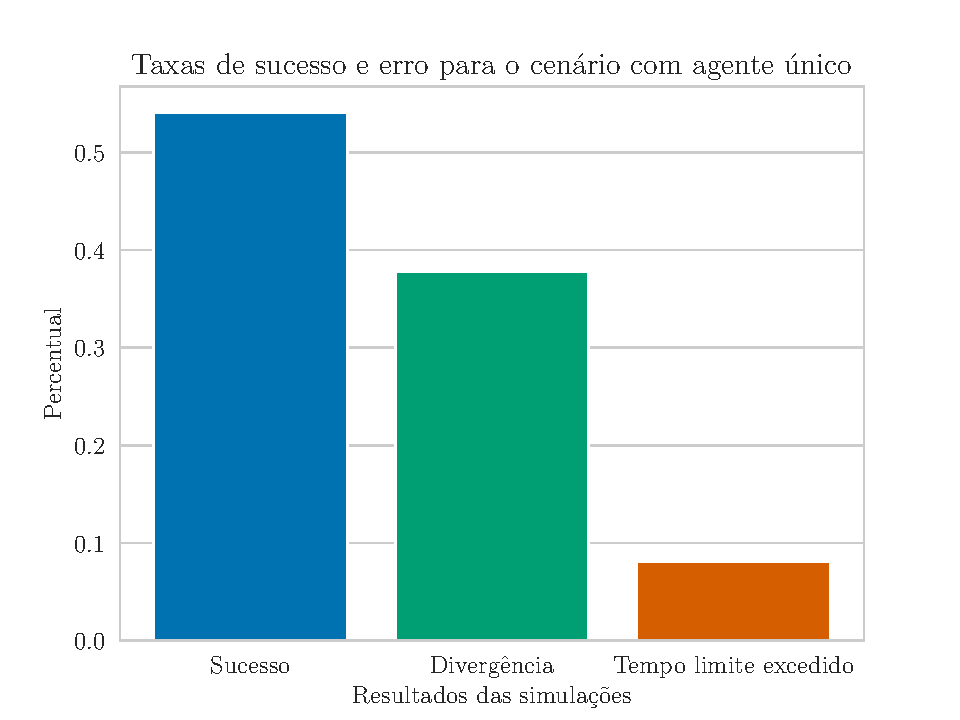
\includegraphics[width=.7\textwidth]{figs/success_rate_bar_single_robot.pdf}
  \caption[Taxas de sucesso e falha para simulações com um único agente]{Taxas de sucesso e falha por tempo limite excedido ou divergência para o cenário com um único agente.}
  \label{fig:exp-single-robot-sucess-rate}
\end{figure}

Com o objetivo de obter-se o desempenho médio do sistema com um único 
agente foi colhido o tempo de mapeamento de cada simulação em que o
robô obteve sucesso, esses dados se encontram nas tabelas \ref{tab:single-agent-experiment-tab1} e \ref{tab:single-agent-experiment-tab2} no Apêndice 
\ref{app:single-agent-data}. A distribuição dos tempos de mapeamento 
registrados encontra-se ilustrada na Figura \ref{fig:time-coverage-single-agent}; o tempo de mapeamento médio foi de 
429 segundos com desvio padrão de 58 segundos. A Figura \ref{fig:single-agent-path} apresenta o caminho percorrido por quatro 
realizações do mapeamento por um único agente.

\begin{figure}
  \centering
  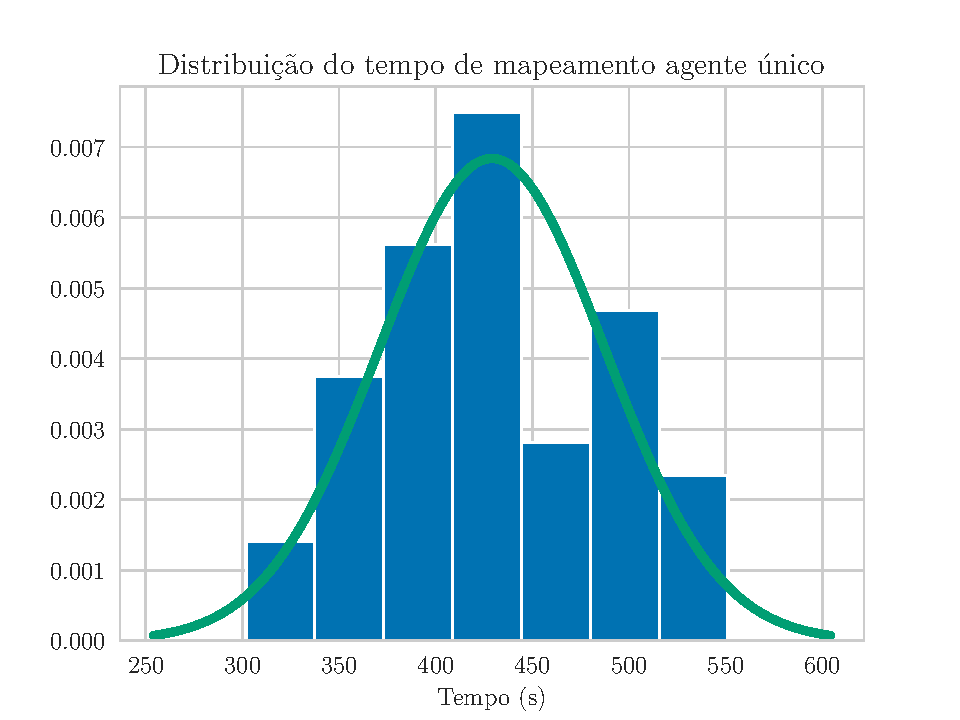
\includegraphics[width=.7\textwidth]{figs/time-coverage-single-agent.pdf}
  \caption[Distribuição do tempo de mapeamento de um único agente]{Histograma de distribuição dos tempos de mapeamento das simulações com um único agente.}
  \label{fig:time-coverage-single-agent}
\end{figure}

\begin{figure}
  \begin{subfigure}{0.49\textwidth}
    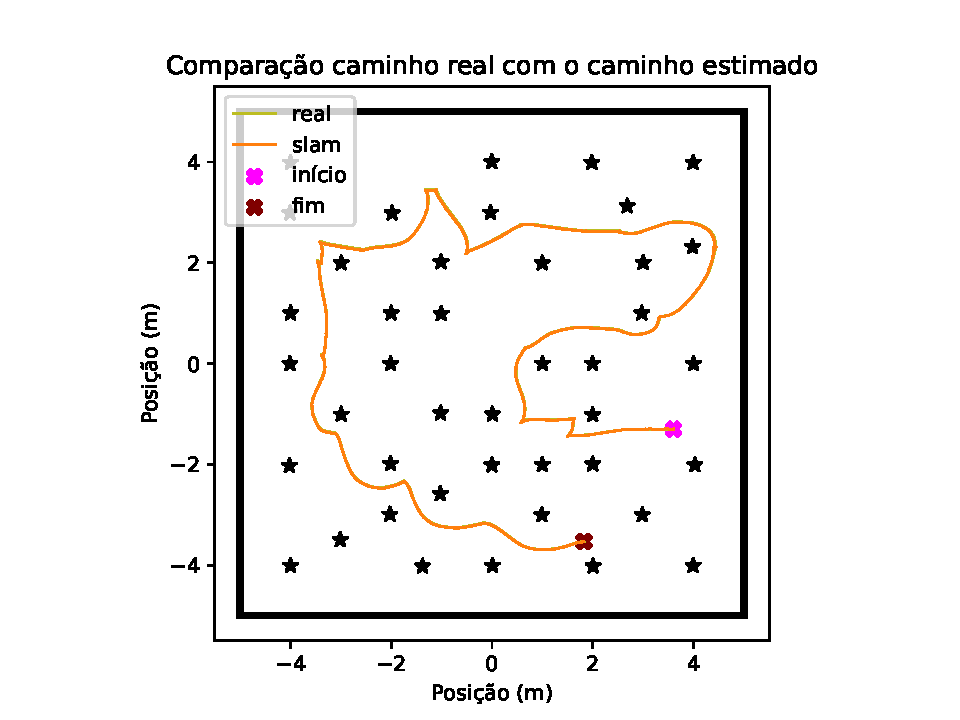
\includegraphics[width=\textwidth]{figs/single-agent/rb1-path-best-time.pdf} 
    \caption{Mapeamento em 302 segundos}
    \label{fig:single-agent-path-best}
  \end{subfigure}
  \begin{subfigure}{0.49\textwidth}
    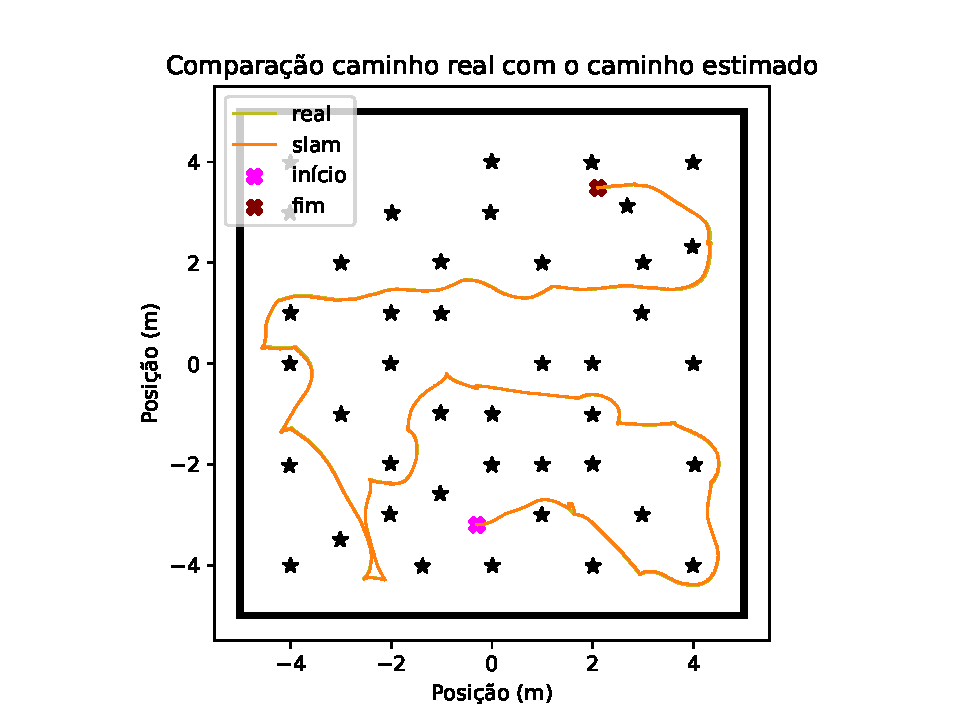
\includegraphics[width=\textwidth]{figs/single-agent/rb1-path-medium-low.pdf} 
    \caption{Mapeamento em 427 segundos}
    \label{fig:single-agente-path-medium-low}
  \end{subfigure}
  \begin{subfigure}{0.49\textwidth}
    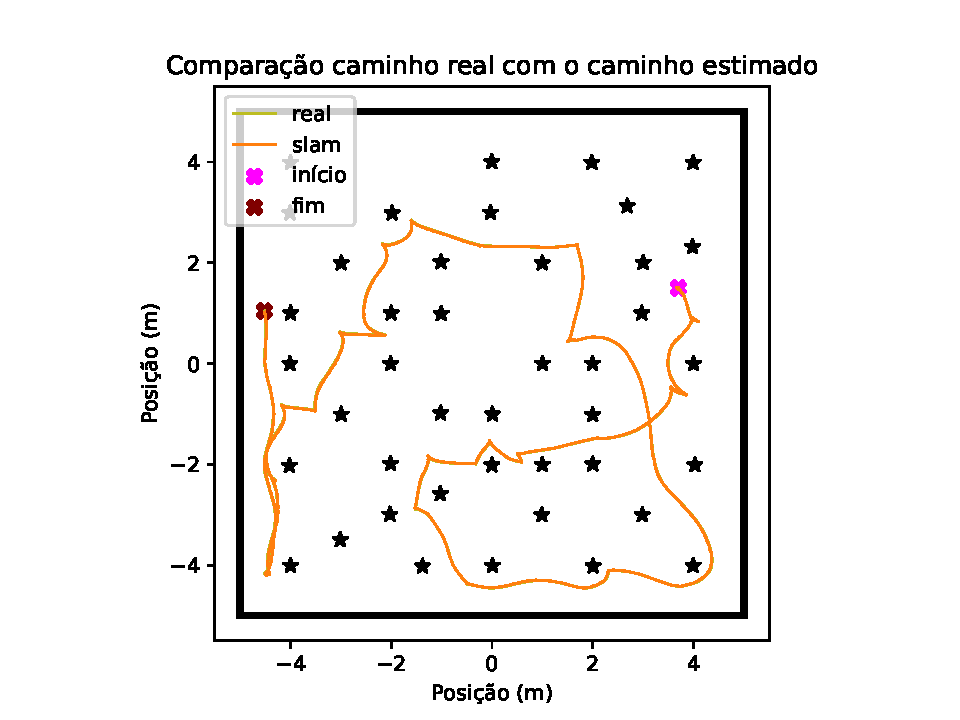
\includegraphics[width=\textwidth]{figs/single-agent/rb1-path-medium-high.pdf} 
    \caption{Mapeamento em 429 segundos}
    \label{fig:single-agent-path-medium-high}
  \end{subfigure}
  \begin{subfigure}{0.49\textwidth}
    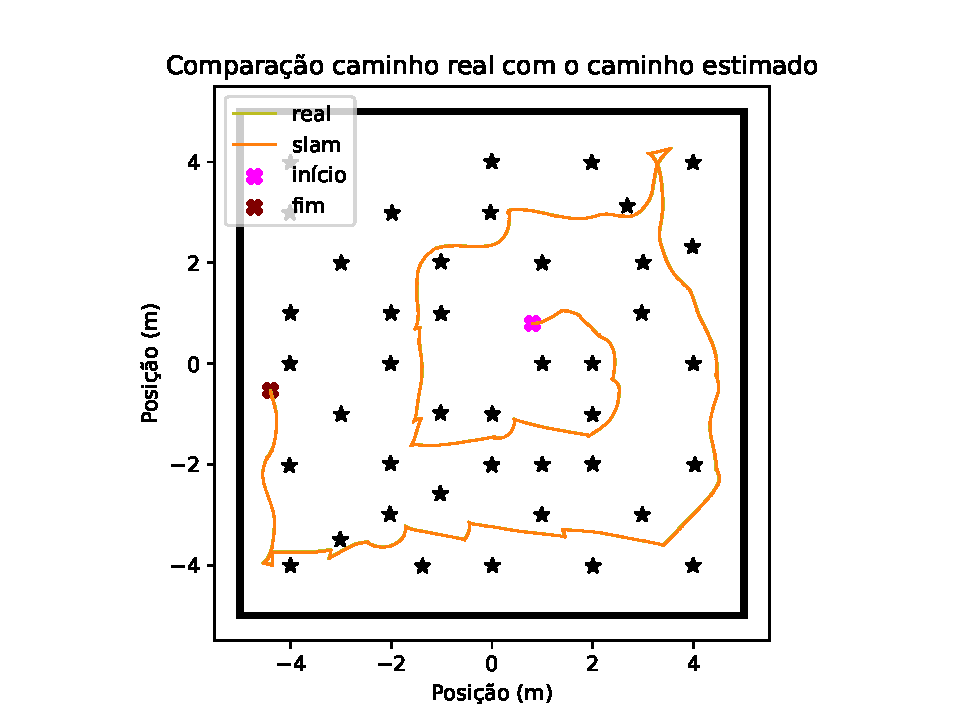
\includegraphics[width=\textwidth]{figs/single-agent/rb1-path-worst.pdf} 
    \caption{Mapeamento em 551 segundos}
    \label{fig:single-agent-path-worst}
  \end{subfigure}
  \caption[Caminhos percorridos durante mapeamento com um único agente]{Caminhos percorridos em diferentes realizações do mapeamento com um único agente em que (a) melhor tempo de mapeamento; (b) realização com tempo levemente inferior ao tempo médio; (c) realização com tempo levemente 
  superior ao tempo médio; (d) pior tempo de mapeamento. Os caminhos 
  real e estimado aparecem sobrepostos na escala da figura. As estrelas representam os pontos de referência (\textit{landmarks}) do ambiente.}
  \label{fig:single-agent-path}
\end{figure}

Durante a realização destes experimentos, criou-se a impressão de que agentes com posição inicial longe das extremidades do ambiente obtinham 
melhor tempo de mapeamento. Para analisar essa hipótese foi feita a Figura \ref{fig:single-agent-initial-pos-and-time}, que relaciona a 
posição inicial do agente com seu tempo de mapeamento através da cor. 

\begin{figure}
  \centering
  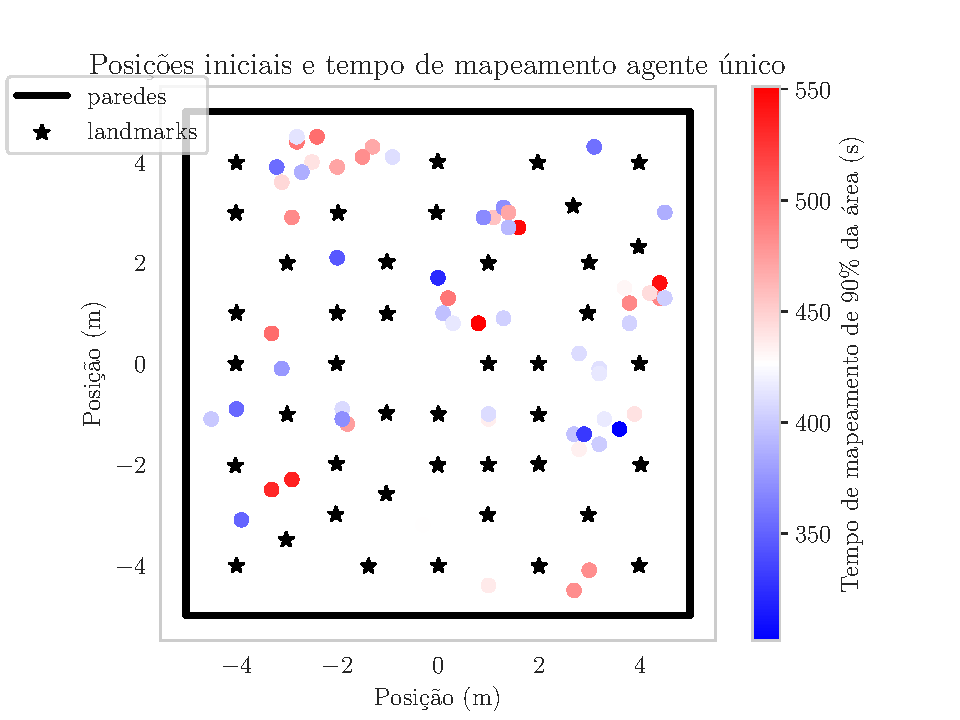
\includegraphics[width=0.7\textwidth]{figs/single-agent/initial_positions_and_time_single_agent.pdf}
  \caption[Posição inicial e tempo de mapeamento das simulações com um único agente.]{Posição inicial e tempo de mapeamento das simulações com um único agente. Cada partícula representa uma posição inicial, o tempo é expressado pela sua cor.}
  \label{fig:single-agent-initial-pos-and-time}
\end{figure}
A Figura confirma essa tendência pois nela é possível notar que a maior parte dos pontos azul claros (representando menor tempo de mapeamento) se 
encontram longe das bordas, enquanto há poucos pontos avermelhados (maior tempo de mapeamento) na região central do mapa.

\section{Mapeamento conjunto e descentralizado}
Esse experimento avalia o cenário com dois robôs desempenhando SLAM 
e trocando mapas entre si como mostrado na Seção \ref{sec:seif-map-exchange}. Como tanto o vetor e a matriz de informação 
quanto as grades de ocupação são compartilhados entre os agentes, esse 
experimento é dividido em duas partes.

Na primeira, o objetivo é medir a 
capacidade dos agentes de trocar os vetores e matrizes de informação 
entre si (Seção \ref{sec:seif-info-exchange}) no cenário ideal onde a
transformação entre seus sistemas de referências é exata e conhecida; para isso são fornecidas as poses iniciais de cada agente. Já 
na segunda parte, os agentes não conhecem suas poses iniciais e usam o 
registro de nuvem de pontos para calcular as transformações.

Nos cenários multiagente, a comunicação ocorre sempre que dois robôs 
chegam a uma distância de dois metros um do outro e há um intervalo 
mínimo de 60 segundos entre duas comunicações consecutivas de um mesmo 
par de robôs. Erros de comunicação ou degeneração de mensagens não são 
simulados.

\subsection{Pose inicial conhecida}
\label{sec:exp-known-initial-pose}
Além do ganho de redundância, sistemas multiagentes também podem 
apresentar ganho de eficiência ao dividir a carga de trabalho entre os 
robôs. Para analisar o desempenho de mapeamento com dois agentes, 
foram realizadas diversas simulações variando a posição inicial dos 
agentes, nos moldes do experimento anterior com um único agente.

Neste experimento foram realizadas 126 simulações, pois, assim como no experimento anterior, o objetivo era realizar aos menos 100 repetições conforme os passos apresentados em \cite[p.~52]{paula2014metodo}; destas, em 46 os 
agentes obtiveram sucesso ao mapear o ambiente sem que a estimação de 
nenhum divergisse, 22 falharam por tempo limite excedido e 58 
falharam por erro de estimação (divergência), o comparativo está na 
Figura \ref{fig:exp-two-robot-sucess-rate}. Os dados das realizações 
que obtiveram sucesso estão registrados nas tabelas \ref{tab:two-agent-experiment-pos-and-time-tab1}, \ref{tab:two-agent-experiment-pos-and-time-tab2}, \ref{tab:two-agent-experiment-iae-tab1} e \ref{tab:two-agent-experiment-iae-tab2} no Apêndice \ref{app:two-agent-data}.

Constata-se então que houve aumento de falhas 
tanto por divergência quanto por tempo limite excedido em comparação 
com o cenário com um único agente. O aumento das falhas por tempo limite 
excedido pode ser explicado pelo aumento de cenários em que a biblioteca de navegação do 
ROS fica presa. Isso ocorre quando um robô fica a uma distância de um obstáculo abaixo de um limiar de segurança e para de se movimentar para evitar uma colisão, sendo que esse problema é mais comum em ambientes dinâmicos \cite{zheng2021ros}. Já o aumento de falhas por divergência do filtro ocorre 
pois a chance de um \emph{ou} outro agente falhar é maior do que a de um único agente.

\begin{figure}
  \centering
  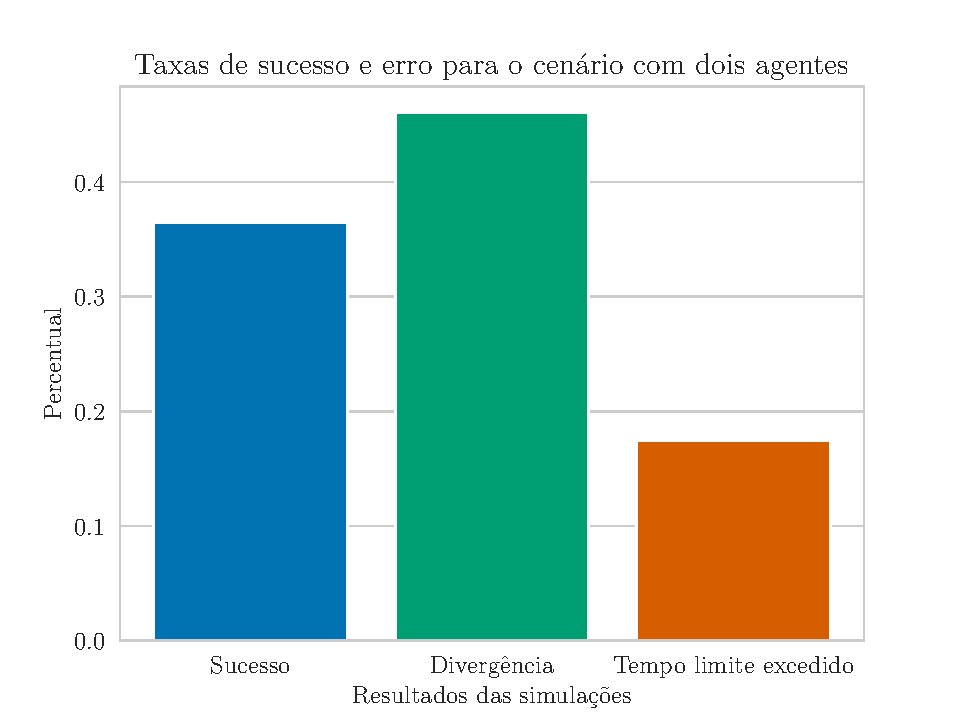
\includegraphics[width=.7\textwidth]{figs/success_rate_bar_two_agents.pdf}
  \caption[Taxas de sucesso e falha para simulações com dois agentes]{Taxas de sucesso e falha por tempo limite excedido ou divergência para o cenário com dois agentes.}
  \label{fig:exp-two-robot-sucess-rate}
\end{figure}

A distribuição do tempo de mapeamento das simulações bem-sucedidas com dois agentes se 
encontra na Figura \ref{fig:time-coverage-two-agents}; o tempo de 
mapeamento médio foi de 321 segundos com desvio padrão de 62 segundos. 
Esse tempo representa 75\% do tempo de mapeamento médio de um único 
agente, mostrado na Figura \ref{fig:time-coverage-single-agent}. A 
relação das posições iniciais, de ambos os robôs em todas as realizações, com o tempo de mapeamento pode ser 
observada na Figura \ref{fig:two-agent-initial-pos-and-time}.  Na Figura \ref{fig:two-agent-path} são também apresentados, como no experimento anterior, 
os caminhos percorridos pelos robôs em quatro realizações das 
simulações com dois agentes.

\begin{figure}
  \centering
  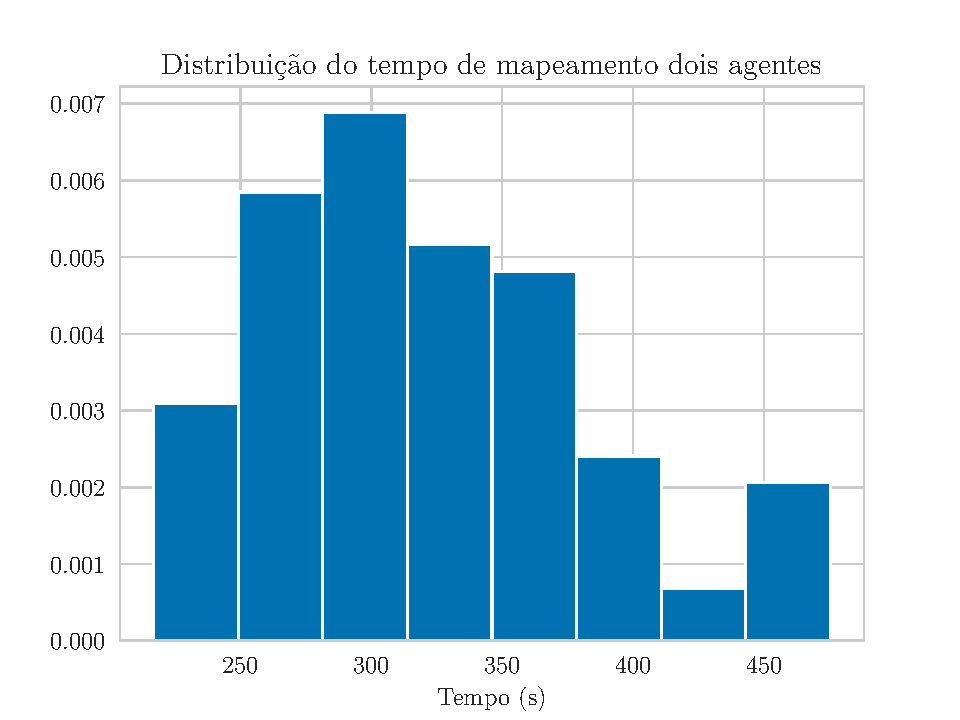
\includegraphics[width=.7\textwidth]{figs/time-coverage_two_agents.pdf}
  \caption[Distribuição do tempo de mapeamento de dois agentes]{Histograma de distribuição dos tempos de mapeamento das simulações com dois agentes.}
  \label{fig:time-coverage-two-agents}
\end{figure}

\begin{figure}
  \centering
  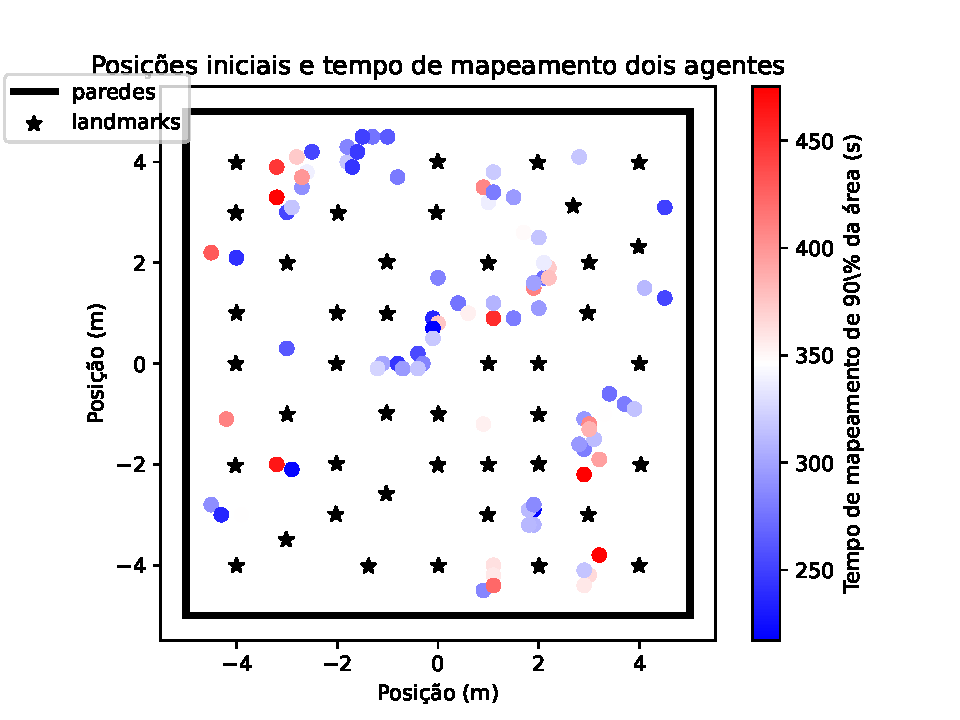
\includegraphics[width=0.7\textwidth]{figs/two-agents/initial_positions_and_time_two_agents.pdf}
  \caption[Posição inicial e tempo de mapeamento das simulações com dois agentes.]{Posição inicial e tempo de mapeamento de ambos os robôs nas simulações com dois agentes. Cada partícula representa uma posição inicial, o tempo é expressado pela sua cor.}
  \label{fig:two-agent-initial-pos-and-time}
\end{figure}

\begin{figure}
  \begin{subfigure}{0.49\textwidth}
    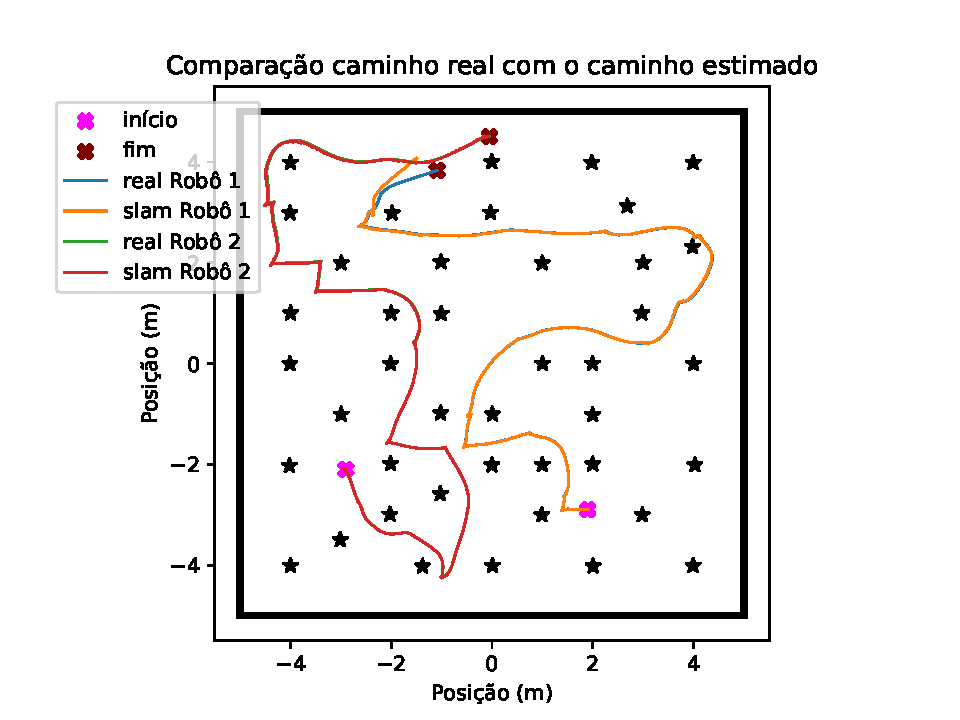
\includegraphics[width=\textwidth]{figs/two-agents/robots-path-best-time.pdf} 
    \caption{Mapeamento médio em 220 segundos}
    \label{fig:two-agent-path-best}
  \end{subfigure}
  \begin{subfigure}{0.49\textwidth}
    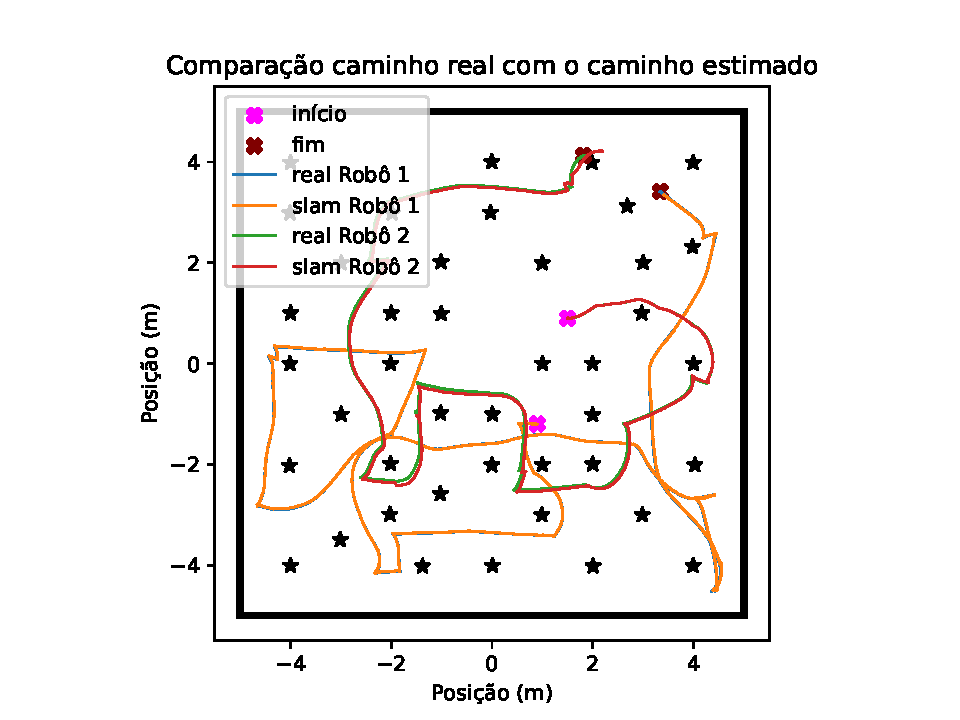
\includegraphics[width=\textwidth]{figs/two-agents/robots-path-medium-low.pdf} 
    \caption{Mapeamento médio em 317 segundos}
    \label{fig:two-agente-path-medium-low}
  \end{subfigure}
  \begin{subfigure}{0.49\textwidth}
    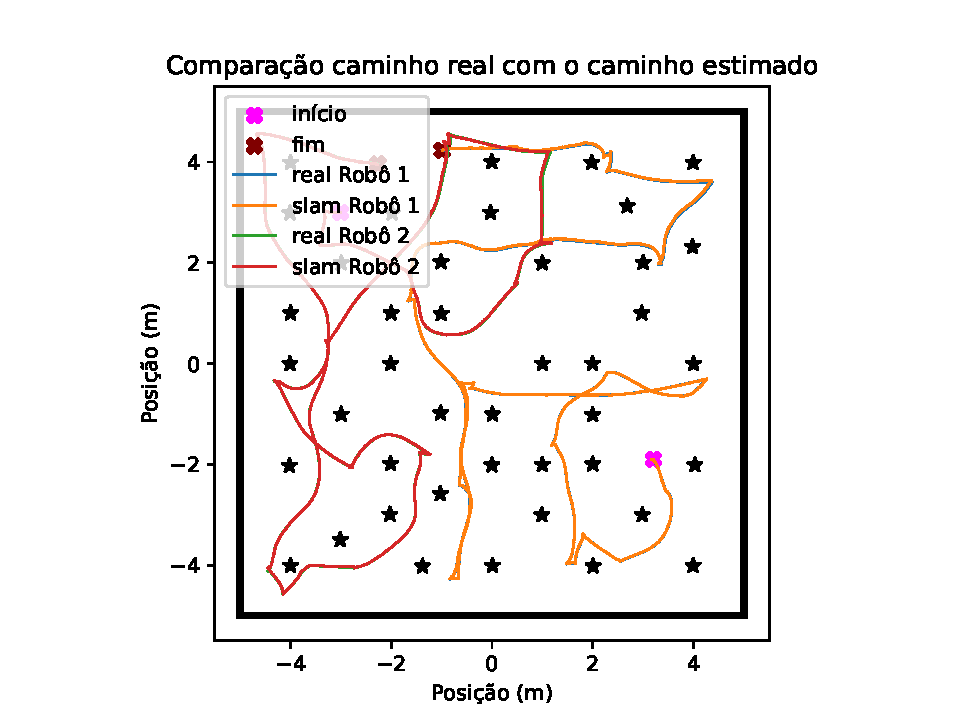
\includegraphics[width=\textwidth]{figs/two-agents/robots-path-medium-high.pdf} 
    \caption{Mapeamento médio em 324 segundos}
    \label{fig:two-agent-path-medium-high}
  \end{subfigure}
  \begin{subfigure}{0.49\textwidth}
    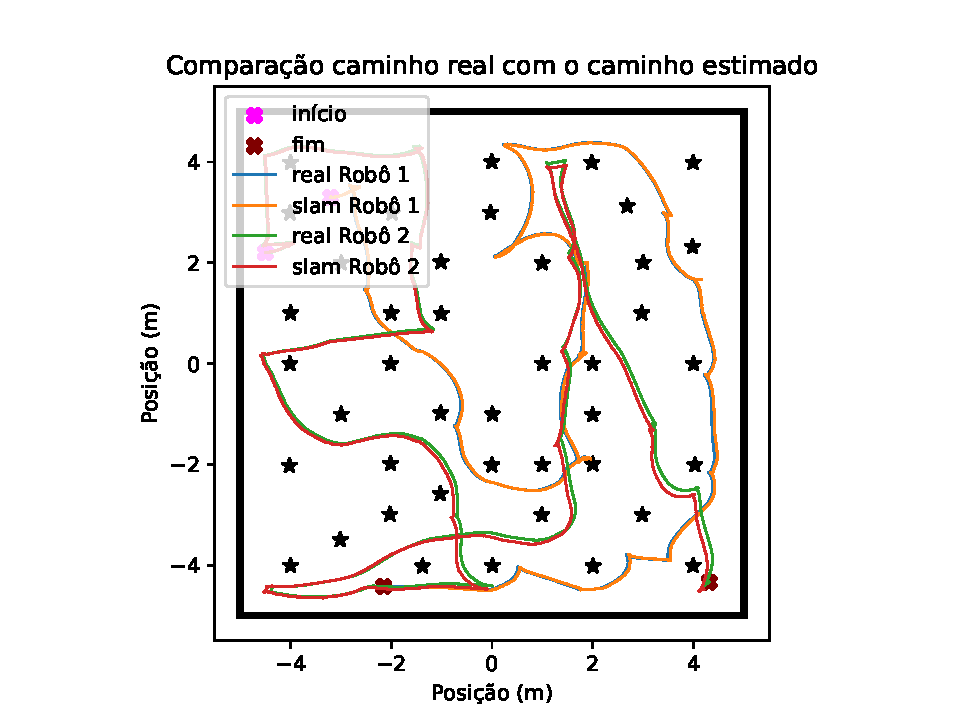
\includegraphics[width=\textwidth]{figs/two-agents/robots-path-worst.pdf} 
    \caption{Mapeamento médio em 451 segundos}
    \label{fig:two-agent-path-worst}
  \end{subfigure}
  \caption[Caminhos percorridos durante mapeamento com dois agentes]{Caminhos percorridos em diferentes realizações do mapeamento com dois agentes em que (a) melhor tempo médio de mapeamento; (b) realização com tempo médio levemente inferior ao tempo médio geral; (c) realização com tempo médio levemente 
  superior ao tempo médio geral; (d) pior tempo de mapeamento. Os caminhos 
  real e estimado podem aparecer sobrepostos na escala da figura. As estrelas representam os pontos de referência (\textit{landmarks}) do ambiente.}
  \label{fig:two-agent-path}
\end{figure}

Embora com o dobro de agentes, o sistema não obteve o dobro do 
desempenho no tempo de exploração. Isso pode ser explicado por dois motivos: o primeiro é que não há uma 
política de exploração conjunta acordada entre os agentes; cada um 
explora o ambiente com base nas fronteiras presentes nos seus mapas 
individuais sem levar em consideração a posição de seu par em relação 
a essas fronteiras; o segundo motivo é que a navegação se torna mais 
complexa, pois agora um agente deve se desviar do outro durante a 
exploração e também não fazem isso de maneira sincronizada e/ou combinada.

% a curva da área coberta pelo tempo é ilustrada na 
% Figura \ref{fig:area-coverage-single-robot}. Logo após o experimento foi repetido no mesmo ambiente com dois e três 
% robôs, as curvas estão ilustradas na Figura \ref{fig:know-initial-pose-area-coverage}.

% \begin{figure}
%   \centering
%   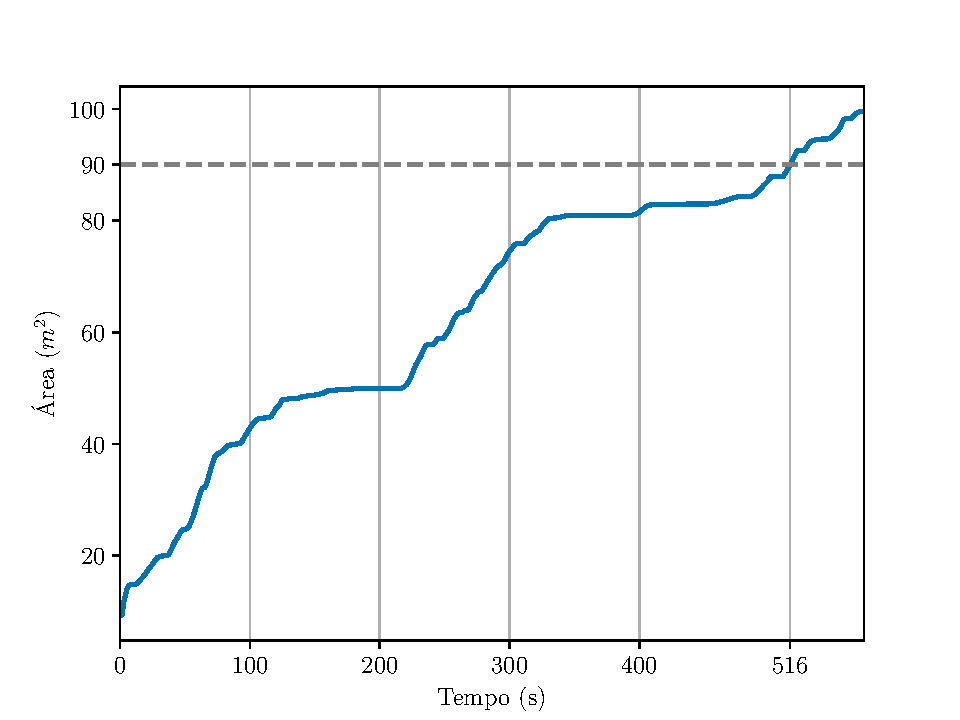
\includegraphics[width=.6\textwidth]{figs/area_coverage_single_robot.pdf}
%   \caption[Evolução da área coberta por um único robô]{Evolução da área coberta ao longo do tempo por um único robô, 
%   no ambiente representado na Figura \ref{fig:environment} com área total 
%   de 100 $m^2$. O robô iniciou na posição $(2.5, 2.5)$, em relação ao centro do ambiente. Os platôs correspondem a intervalos nos quais o robô está atravessando uma área já mapeada para explorar uma nova fronteira.}
%   \label{fig:area-coverage-single-robot}
% \end{figure}

% \begin{figure}
%   \centering
%   \begin{subfigure}{0.49\textwidth}
%     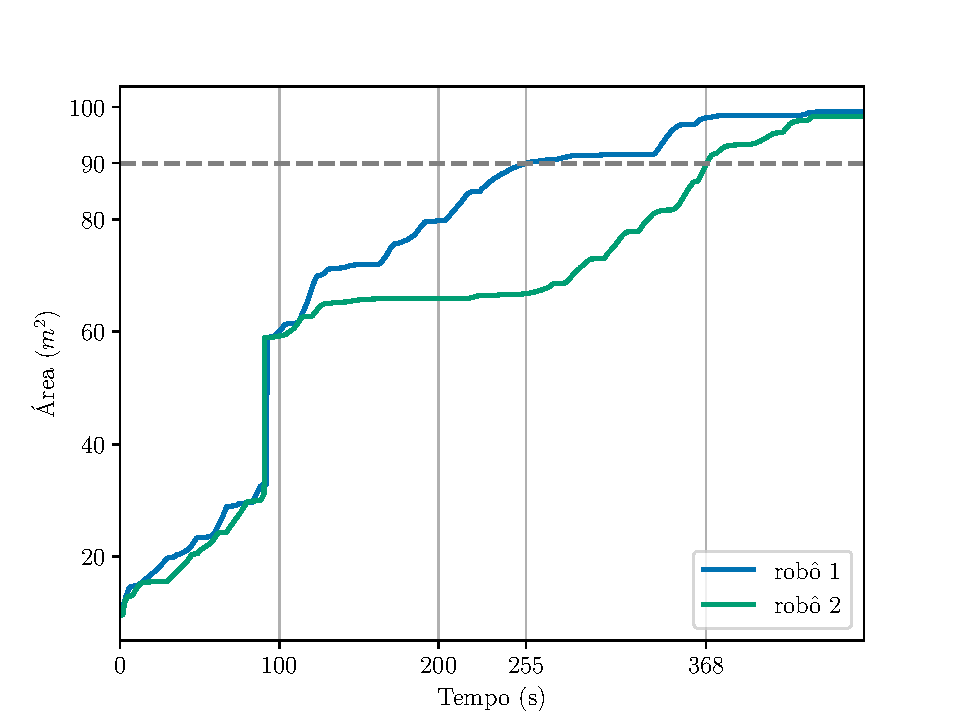
\includegraphics[width=\textwidth]{figs/area_coverage_two_robots-with-known-positions.pdf}
%     \caption{Evolução da área coberta ao longo do tempo por dois robôs. 
%     }
%     \label{}
%   \end{subfigure}
%   \hfill
%   \begin{subfigure}{0.49\textwidth}
%     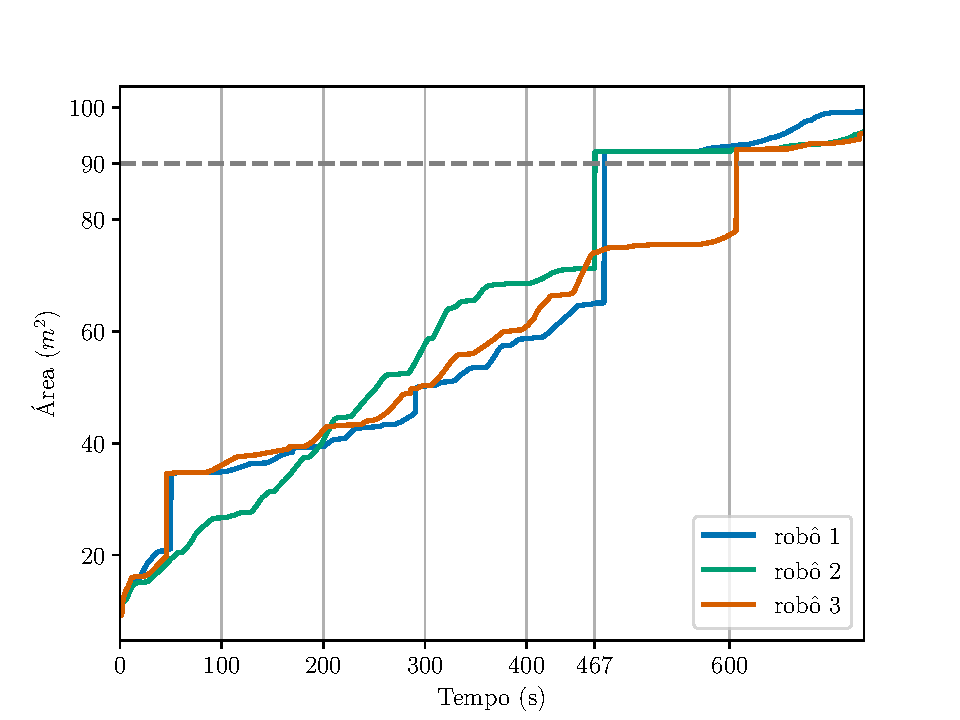
\includegraphics[width=\textwidth]{figs/area_coverage_three_robots-with-known-positions.pdf}
%     \caption{Evolução da área coberta ao longo do tempo por três robôs. }
%     \label{}
%   \end{subfigure}
%   \caption[Comparação da evolução das áreas cobertas por dois e três agentes com pose inicial conhecida]{Evolução da área coberta por dois e três agentes com pose inicial conhecida. Os momentos de comunicação e troca de mapas entre os agentes podem ser identificados por saltos verticais nas curvas de área coberta por cada agente.}
%   \label{fig:know-initial-pose-area-coverage}
% \end{figure}

% A Tabela \ref{table:multiagent-exploration-know-initial-pose} registra o momento em que todos os agentes 
% dos diferentes sistemas alcançam a marca de 90\% de área mapeada. Como é 
% possível notar, quando houve ganho de eficiência com dois robôs ele não fez o tempo 
% cair pela metade. E, ainda no cenário com três robôs, esse ganho foi negativo; o sistema levou mais tempo que o sistema com um único agente. 
% Isso pode ser explicado por dois motivos: o primeiro é que não há uma 
% política de exploração conjunta acordada entre os agentes; cada um 
% explora o ambiente com base nas fronteiras presentes nos seus mapas 
% individuais sem levar em consideração a posição de seus pares em relação 
% a essas fronteiras; o segundo motivo é que a navegação se torna mais 
% complexa pois agora um agente deve se desviar do outro durante a 
% exploração e também não fazem isso de maneira sincronizada e/ou combinada.

% \begin{table}[]
% \center
% \caption{Comparação entre o tempo levado para atingir a marca de 90\% de área coberta, de um ambiente de 100 $m^2$, entre os sistemas de múltiplos agentes e agente único.}
% \label{table:multiagent-exploration-know-initial-pose}
% \begin{tabularx}{\textwidth}{@{}YYY@{}}
% \hline
% Quantidade de agentes & Tempo para 90\% de área coberta (s) & Eficiência em relação a um agente \\ \hline
% 1 & 516 & - \\
% 2 & 368 & +40.21\% \\
% 3 & 600 & -14\% \\ \hline
% \end{tabularx}
% \end{table}

% Apesar do ganho ficar abaixo do 
% esperado, observando as Figuras \ref{fig:area-coverage-single-robot} e 
% \ref{fig:know-initial-pose-area-coverage} é possível ver que o tempo 
% levado pelo primeiro agente dos sistemas multiagentes para atingir a 
% marca de 90\% de área coberta foi sempre menor que o tempo levado 
% pelo sistema de agente único, com destaque para o sistema de dois agentes 
% no qual o primeiro agente atingiu a marca em menos da metade do tempo 
% do sistema de agente único.


\subsection{Pose inicial desconhecida}
\label{sec:exp-unknown-initial-pose}
Nesse último experimento, as poses iniciais dos agentes não foram 
fornecidas, como no experimento anterior. Dessa forma para incorporarem 
um o mapa do outro é necessário que calculem a transformação entre seus 
mapas de \textit{landmarks} utilizando a técnica de registro de nuvem de 
pontos discutida na Seção \ref{sec:point-cloud-registration}. A Figura 
\ref{fig:unknown-initial-pose-area-coverage} mostra duas simulações do 
sistema SLAM com dois robôs; entre elas variou-se apenas as posições 
iniciais dos agentes.

\begin{figure}
  \centering
  \begin{subfigure}{0.49\textwidth}
    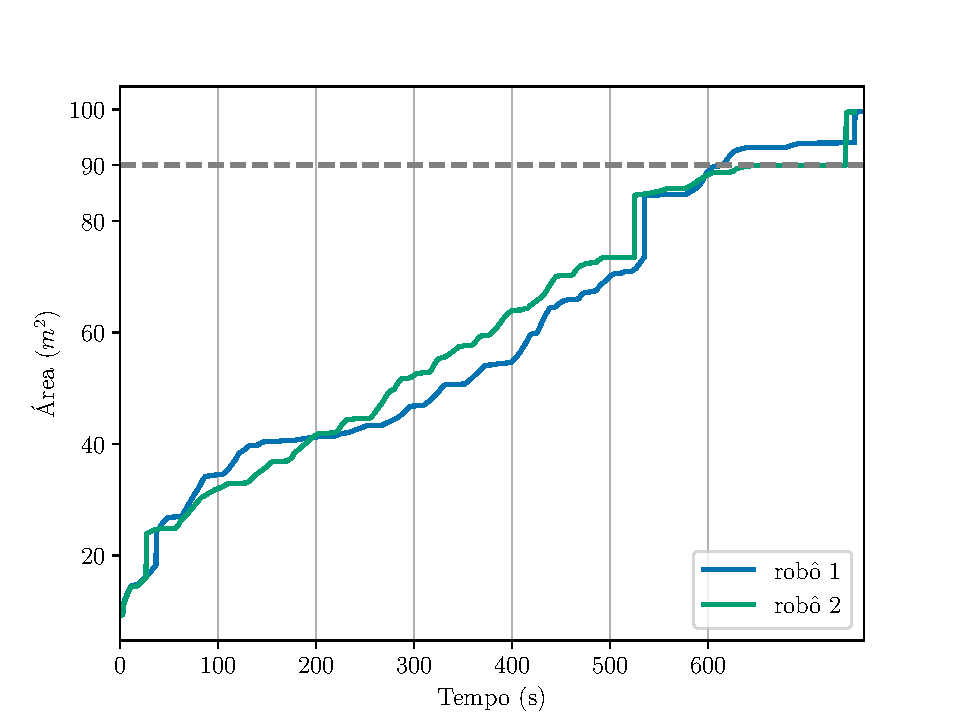
\includegraphics[width=\textwidth]{figs/area_coverage_two_robots-with-unknown-positions-01.pdf}
    \caption{}
    \label{fig:unk-pose-area-coverage-first}
  \end{subfigure}
  \hfill
  \begin{subfigure}{0.49\textwidth}
    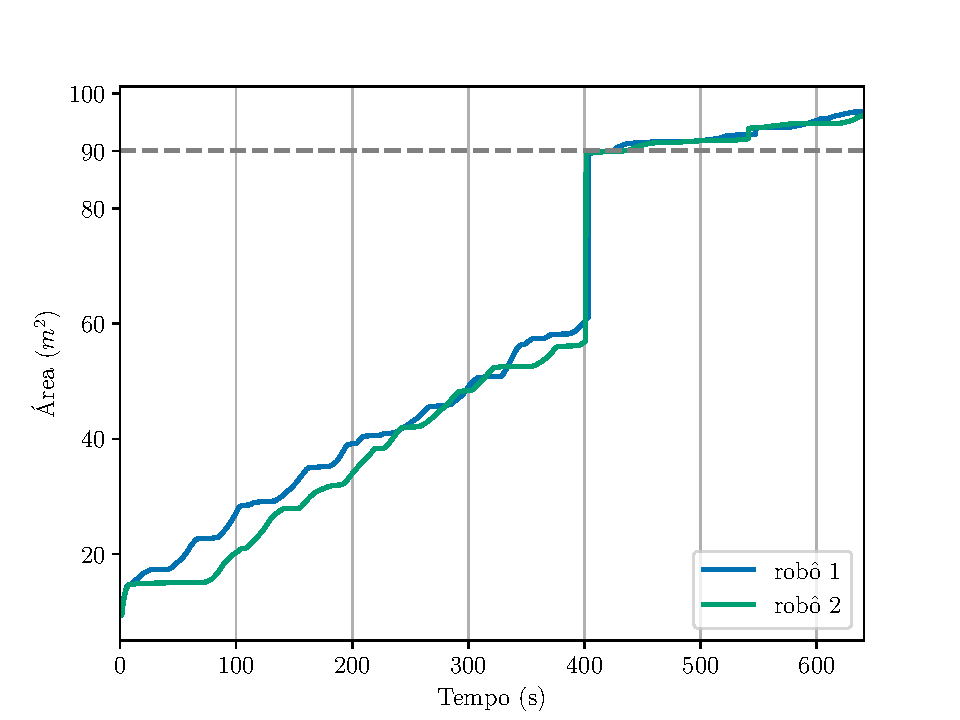
\includegraphics[width=\textwidth]{figs/area_coverage_two_robots-with-unknown-positions-02.pdf}
    \caption{}
    \label{fig:}
  \end{subfigure}
  \caption[Comparação da evolução das áreas cobertas por dois agentes com pose inicial desconhecida]{Diferentes execuções do mapeamento com dois agentes com pose inicial desconhecida. Entre as execuções variou-se a pose inicial dos 
  agentes. As curvas da Figura da direta estão defasadas, pois o segundo 
  agente foi colocado no ambiente alguns instantes depois que o primeiro. Isso ocorreu pois neste experimento especificamente o processo de inicialização da simulação foi feito manualmente, o que provocou diferença no tempo em que os agente foram colocados no ambiente.}
  \label{fig:unknown-initial-pose-area-coverage}
\end{figure}

Além dos problemas de sincronia entre os agentes, já citados no experimento 
anterior, neste exemplo também foram observados problemas com a estimação 
da transformação entre os mapas de \textit{landmarks} dos agentes. 
Enquanto no experimento anterior a troca de mapas entre os robôs sempre 
ocorre com sucesso, pois eles sabem suas poses iniciais e, portanto, sabem 
relacionar o mapa de um com o do outro, neste experimento nem toda aproximação dos 
robôs resultou em troca dos mapas, pois muitas vezes eles não conseguiram 
estimar a transformação.

Este experimento também teve que ser repetido mais de uma vez, pois em 
muitas execuções os robôs estimavam a transformação errada, incorporando 
a informação do outro robô de maneira errada e provocando divergência do 
filtro. Desse modo, a técnica de registro de nuvem de pontos utilizada 
não se mostrou robusta para estimar a transformação entre os mapas dos robôs. Por conta da alta taxa de falha na estimação da transformação 
relativa, que leva à divergência, não foram feitas realizações 
repetidas neste experimento para avaliar o desempenho.

